\chapter{\label{par_est}Parameter estimation using SOAP}
%%%%%%%%%%%%
%%%%%%%%%%%%
%%%%%%%%%%%%
%%%%%

Throughout Sec.~\ref{soap} and \ref{machine} we developed techniques which could identify whether a potential signal is present within a small frequency band ($0.1 Hz$) and return the most likely frequency track if the signal in that band.
This is useful information for all-sky searches as it can limit the parameter space for deeper searches such as those described in Sec.~\ref{searchcw:search:targeted}. 
However, this only limits the parameters space to a smaller frequency band, and potentially the frequency and derivative if we used the Viterbi track information.
This still leaves a large parameter space which a more sensitive method would have to search through.
In particular the sky position of the source has to be sampled finely as \gls{LIGO} can accurately localise a \gls{CW} source.
This is because the source is observed at multiple positions as the earth orbits sun, giving an effective aperture of the earth's orbital radius.
The SOAP search would therefore benefit if it could provide more information on the astrophysical source.

In this chapter I will outline a Bayesian method which uses the output Viterbi tracks of the SOAP search in Sec.~\ref{soap} to return some astrophysical parameters of a source.
Sec.~\ref{par_est:freq} will outline the model of the frequency evolution of a \gls{CW} from a source with a slowly varying frequency,
Sec.~\ref{par_est:bayes} will outline the Bayesian model for this analysis and Sec.~\ref{par_est:results} will show the results from testing on simulated signals.

%%%%
%%%%
\section{\label{par_est:freq}Pulsar frequency evolution}
%%%%
%%%%

The SOAP search returns a Viterbi track, where if this track follows the frequency of a pulsar signal, frequency evolution contains information of the sky position ($\alpha, \delta$) and the frequency of the source $f$ and its derivative $\dot{f}$ where we ignore higher order frequency derivatives.
From the Viterbi track, we should then be able to extract this information as we have a model for the phase evolution (and therefore frequency evolution) of the source described in Eq.~\ref{searchcw:model:phase} in Sec.~\ref{searchcw:model}.
To relate this phase evolution to the sky position parameters, we can look closer at Eq.~\ref{searchcw:model:ssbtime}, where we describe the shift in arrival time due to the earths motion. 

The second term in Eq.~\ref{searchcw:model:ssbtime} describes the Doppler shift due to the earth's orbit and rotation.
Where the $\bm{r}$ is the position of the detector and $\bm{n}$ is a unit vector in the direction of the source. 
As in \citep{schutz1998DataAnalysis}, we use the coordinate frame in the \gls{SSB} where the $z$ axis is perpendicular to the ecliptic and the $x$ axis is parallel to the celestial sphere.
In this frame the unit vector pointing towards the star can be written as 
\begin{equation}
    \label{par_est:freq:unit}
    \bm{n} = 
    \left(
    \begin{matrix}
        1 & 0 & 0  \\
        0 & \cos \epsilon & \sin \epsilon \\
        0 & -\sin \epsilon & \cos \epsilon \\
    \end{matrix} \right)
    \left(
    \begin{matrix}
        \cos(\alpha)\cos(\delta)  \\
        \sin(\alpha)\cos(\delta) \\
        \sin(\delta) \\
    \end{matrix} \right),
\end{equation}
where $\alpha$ and $\delta$ are the right ascension and declination (sky position) of the source and $\epsilon$ is the angle between the ecliptic and the earth's equator.
The first matrix in Eq.~\ref{par_est:freq:unit} describes a rotation from the \joe{earths} frame where $\alpha$ and $\delta$ are measured to the \gls{SSB} frame. 
The second matrix transforms the sky position parameters to their component $x,y,z$ coordinates.

The position vector of the earth at a time $t$, $\bm{r}$ in Eq.~\ref{searchcw:model:ssbtime}, can split into the addition of two components, the position due to the orbit of the earth and position due to the rotation of the earth.
The position of the earth in its orbit is described in cartesian coordinates as
\begin{equation}
    \bm{r}_{orb} = R_{\mathrm{O}}
    \left(
    \begin{matrix}
        \cos{\left( \Omega_{\mathrm{O}} t + \phi_{\omega){O}}  \right)}  \\
        \sin{\left( \Omega_{\mathrm{O}} t + \phi_{\omega){O}}  \right)} \\
        0 \\
    \end{matrix} \right),
\end{equation}
where $R_{\mathrm{O}}$ is the radius of the earth's orbit (1 AU), $\Omega_{\mathrm{O}}$ is the angular frequency of the earth's orbit $2\pi/T_{\mathrm{O}}$, where $T_{\mathrm{O}}$ is one year and $\phi_{\omega){O}}$ is some phase which defines the position of the earth in its orbital motion.
The position due to the rotation of the earth can then be described by 
\begin{equation}
    \bm{r}_{rot} = R_{\mathrm{R}}
    \left(
    \begin{matrix}
        1 & 0 & 0  \\
        0 & \cos \epsilon & \sin \epsilon \\
        0 & -\sin \epsilon & \cos \epsilon \\
    \end{matrix} \right)
    \left(
    \begin{matrix}
        \cos{(\lambda)}\cos{\left( \Omega_{\mathrm{R}} t + \phi_{\omega){R}}  \right)}  \\
        \cos{(\lambda)}\sin{\left( \Omega_{\mathrm{R}} t + \phi_{\omega){R}}  \right)} \\
        \sin{(\lambda)} \\
    \end{matrix} \right),
\end{equation}
where $R_{\mathrm{R}}$ is the radius of the earth, $\Omega_{\mathrm{R}}$ is the angular frequency of the earth's rotation $2\pi/T_{\mathrm{R}}$, where $T_{\mathrm{R}}$ is one day, $\phi_{\omega){O}}$ is some phase which defines the position of the earth in its rotational motion and $\lambda$ is the latitude of the detectors site.
These two components can then be added to find the location of the detector in the \gls{SSB} frame
\begin{equation}
    \bm{r} = \bm{r}_{orb} + \bm{r}_{rot}.
\end{equation}

We can now describe the phase evolution of the signal at the detectors site from just the sky position ($\alpha, \delta$) and frequency and its derivative $f,\dot{f}$. 
The frequency of a pulsars signal at any point on the frequency track is then defined by the derivative of the phase with respect to time
\begin{equation}
    f = \frac{d\Phi}{dt}, 
\end{equation}
where $\Phi$ is defined in Eq.~\ref{searchcw:model:phase}.
\joe{maybe add the actual frequency evolution equation}

%
%
\section{\label{par_est:bayes}Bayesian Model}
%
%

As described in Sec.~\ref{par_est:freq} we have a model of a pulsars frequency evolution and we have our Viterbi track which is our observation of a frequency track.
We would now like to estimate the parameters $\bm{\theta} = \left\{\alpha, \delta, f, \dot{f} \right\}$ of a pulsar given that we have observed the frequency track $\bm{V}$.
To do this we use a Bayesian model, where the idea was introduced in Sec.~\ref{intro:prob:bayes}, where we rewrite Bayes formula in terms of this problem
\begin{equation}
    \label{par_est:bayes:eqn}
    p(\bm{\theta} \mid \bm{V}, I) = \frac{p(\bm{\theta}) p(\bm{V} \mid \bm{\theta}, I)}{p(\bm{V} \mid I)}
\end{equation}
where $p(\bm{\theta} \mid \bm{V}, I)$ is the posterior which we are interested in, $p(\bm{\theta})$ is the prior, $p(\bm{V} \mid \bm{\theta}, I)$ is the likelihood and $\bm{V} \mid I)$ is the evidence.
The following sections will describe how we set up the prior and likelihood for this problem.

%
%
\subsection{\label{par_est:bayes:likelihood}Likelihood}
%
%

The likelihood describes how the noise of the data is distributed, i.e. if we subtracted the model frequency track from our observed frequency track, what is the distribution of these values.
If the simulated pulsar signal has an infinitely large \gls{SNR} then the Viterbi track would follow the pulsars frequency track exactly, which would leave a noise distribution of 0 with no variance. 
If conversely, the \gls{SNR} was zero then the Viterbi track would wander randomly through the frequency band and the noise would have a large variance in frequency.
The noise distribution of a Viterbi track, is then dependent on the \gls{SNR} if the signal within the band.
As the distribution of the noise is unknown analytically, we calculate it empirically using many simulated signals.

In Sec.~\ref{soap:results} we generated $\mathcal{O}(10^{4})$ simulated signal which, amongst other quantities, saved the Viterbi track, the simulated pulsar frequency track and the signals \gls{SNR}, $\rho$.
These simulations had \glspl{SNR} between 50 and 150, \joe{might update to 20-200}.
We can estimate the noise distribution by taking the \gls{KDE} of the differences between the Viterbi and pulsar frequency tracks for all simulations in a given \gls{SNR} range.
We split the likelihood into 90 discrete bins, each of which are \gls{SNR} 2 wide, where this ranges from \gls{SNR} 20 to 200.
Figure \ref{par_est:bayes:likelihood:kde142} shows an example of the \glspl{KDE} of a subset of the likelihood bins. 
The sharp peaks in the center of each sub plot in Fig.~\ref{par_est:bayes:likelihood:kde142} represents simulations where the Viterbi track is close to the simulated pulsar track, and the broader distributions represent areas of the Viterbi track has not identified the pulsar track but is wandering randomly.
The sub plots in Fig.~\ref{par_est:bayes:likelihood:kde142} show that as the \gls{SNR} increases the distribution is more closely centred around 0, i.e. the Viterbi and pulsar tracks are similar, which is expected.
%
\begin{figure}[hpt]

    \centering
    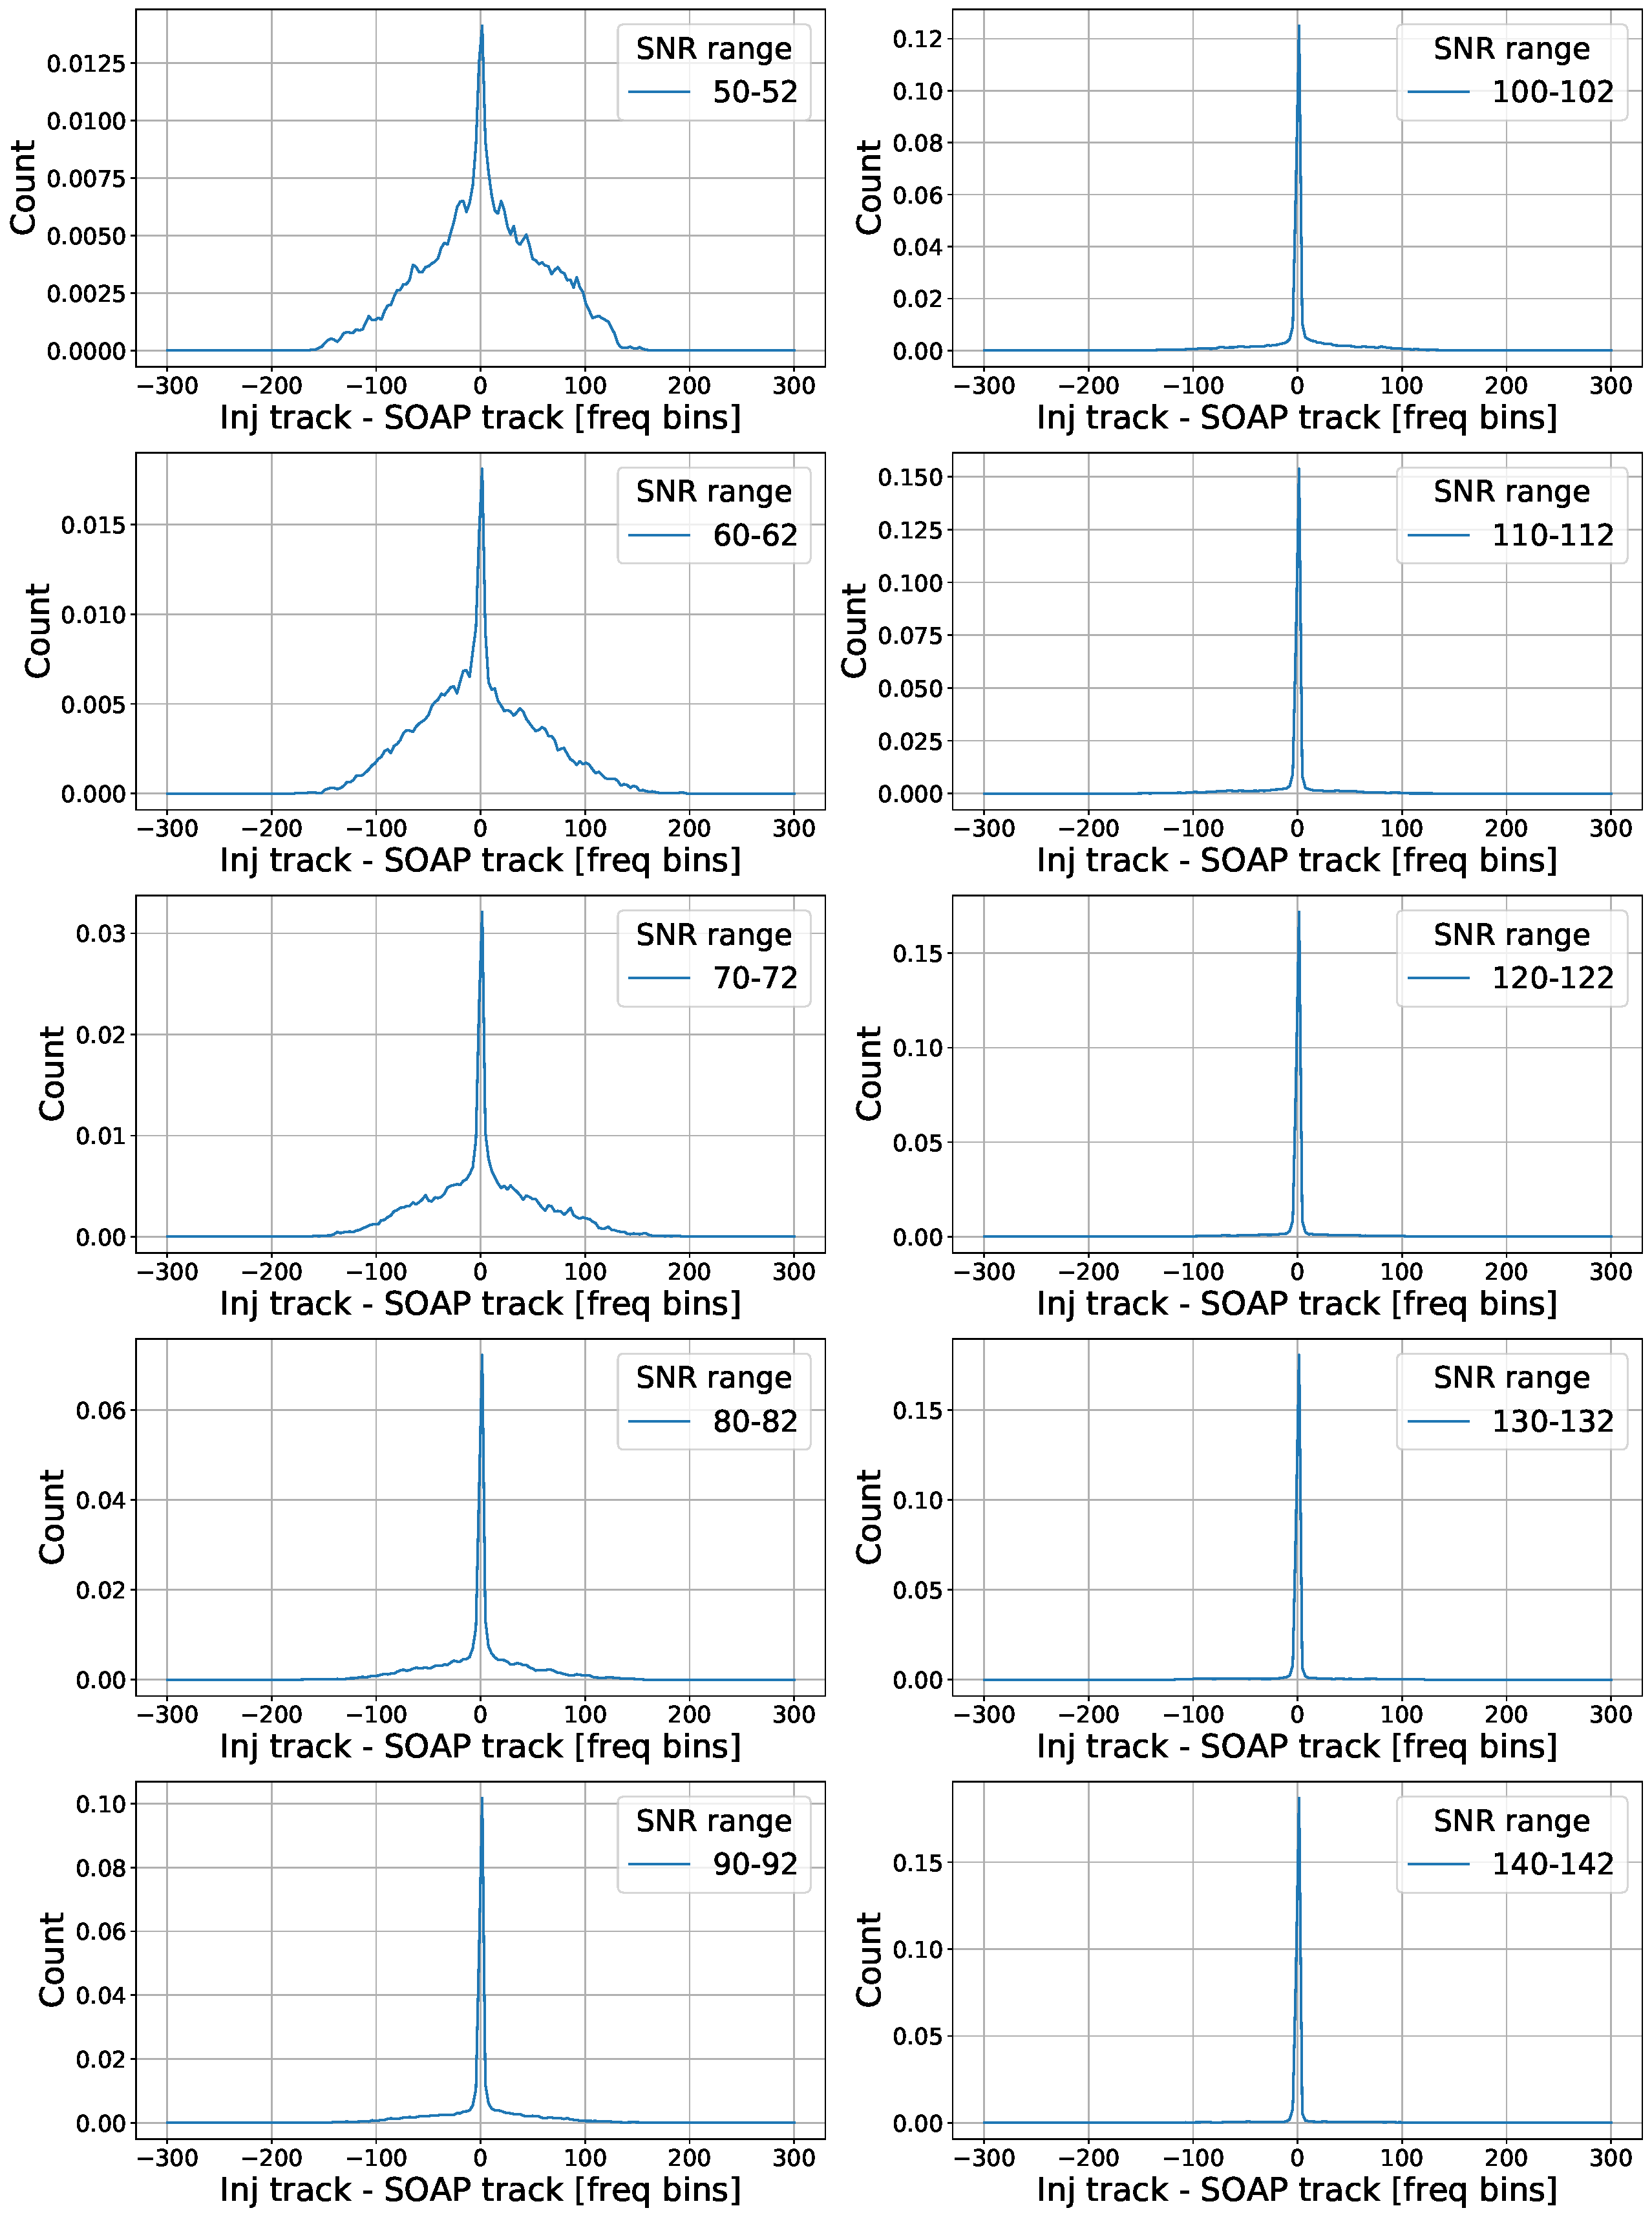
\includegraphics[width=\linewidth]{C5_parameter/KDE_range_50_100.pdf}
    \caption[KDE of likelihood in different \gls{SNR} ranges]{This figure shows the \gls{KDE} estimates of the probability density of the differences between the simulated (injected) pulsar frequency track and the recovered Viterbi track for a number of \gls{SNR} ranges. The difference in the tracks is measured in discrete frequency bins. Each \gls{KDE} is generated from $\sim 300$ simulations which each have $\sim 400$ elements in their frequency tracks. This shows a subset of the binned likelihoods between the range of \gls{SNR} 50 and 150.}
    \label{par_est:bayes:likelihood:kde142}
    
    \end{figure}
%

This does introduce one more parameter to search over in out Bayesian model, which is the \gls{SNR} ($\rho$) of the signal.
These \glspl{KDE} are the used as the likelihood function $p(\bm{V} \mid \bm{\theta}, I)$ in the Bayesian model in Eq.~\ref{par_est:bayes:eqn}, where we not have five parameters $\bm{\theta} = \left\{\alpha, \delta, f, \dot{f} , \rho \right\}$.


%
\subsection{Prior}
%
We set up a simple prior which does not assume much about the parameters, other than limits on their range. 
We use a flat prior for $\alpha$ between $[0,2\pi]$, a flat prior in $\sin{\delta}$ between [-1,1], a flat prior in $f$ in the range of the 0.1 Hz wide sub-band which SOAP searched through and a flat prior in the frequency derivative in the range $[-1\cdot 10^{9},1\cdot 10^{9}]$.
The prior for $\rho$ is also flat in the range $[50,200]$.


\clearpage

%%%%
%%%%
\section{\label{par_est:results}Results}
%%%%
%%%%

The method described in Sec.~\ref{par_est:bayes} takes in a Viterbi track and uses this to estimate the five dimensional posterior distribution $p\left(\left\{ \alpha, \delta, f, \dot{f}, \rho \right\} \mid \bm{V}, I \right)$.
To calculate this posterior we use a technique known as nested sampling, specifically the package {\it Dynesty} \citep{speagle2019DynestyDynamic}. \joe{explain more in the return of intro chapter}

As an example, we can simulate a \gls{CW} signal with neutron star parameters 
\begin{equation}
    \begin{split}
        \alpha &= 4.95 \; \rm{rad}\\
        \delta &= -0.18 \; \rm{rad} \\
        f &= 154.04 \; \rm{Hz}\\
        \dot{f} &= -1.22e-10 \; \rm{Hz s^{-1}}\\
        \rho &= 144,\\
    \end{split}
\end{equation}
and generate the associated spectrograms for the \gls{LIGO} detectors H1 and L1.
The SOAP search from Sec.~\ref{soap} is then run using the line-aware statistics the same parameters as in Sec.~\ref{soap:results}, the output Viterbi track is then plotted with the neutron stars frequency track in Fig.~\ref{par_est:results:freqtrack}.
%
\begin{figure}[pt]

    \centering
    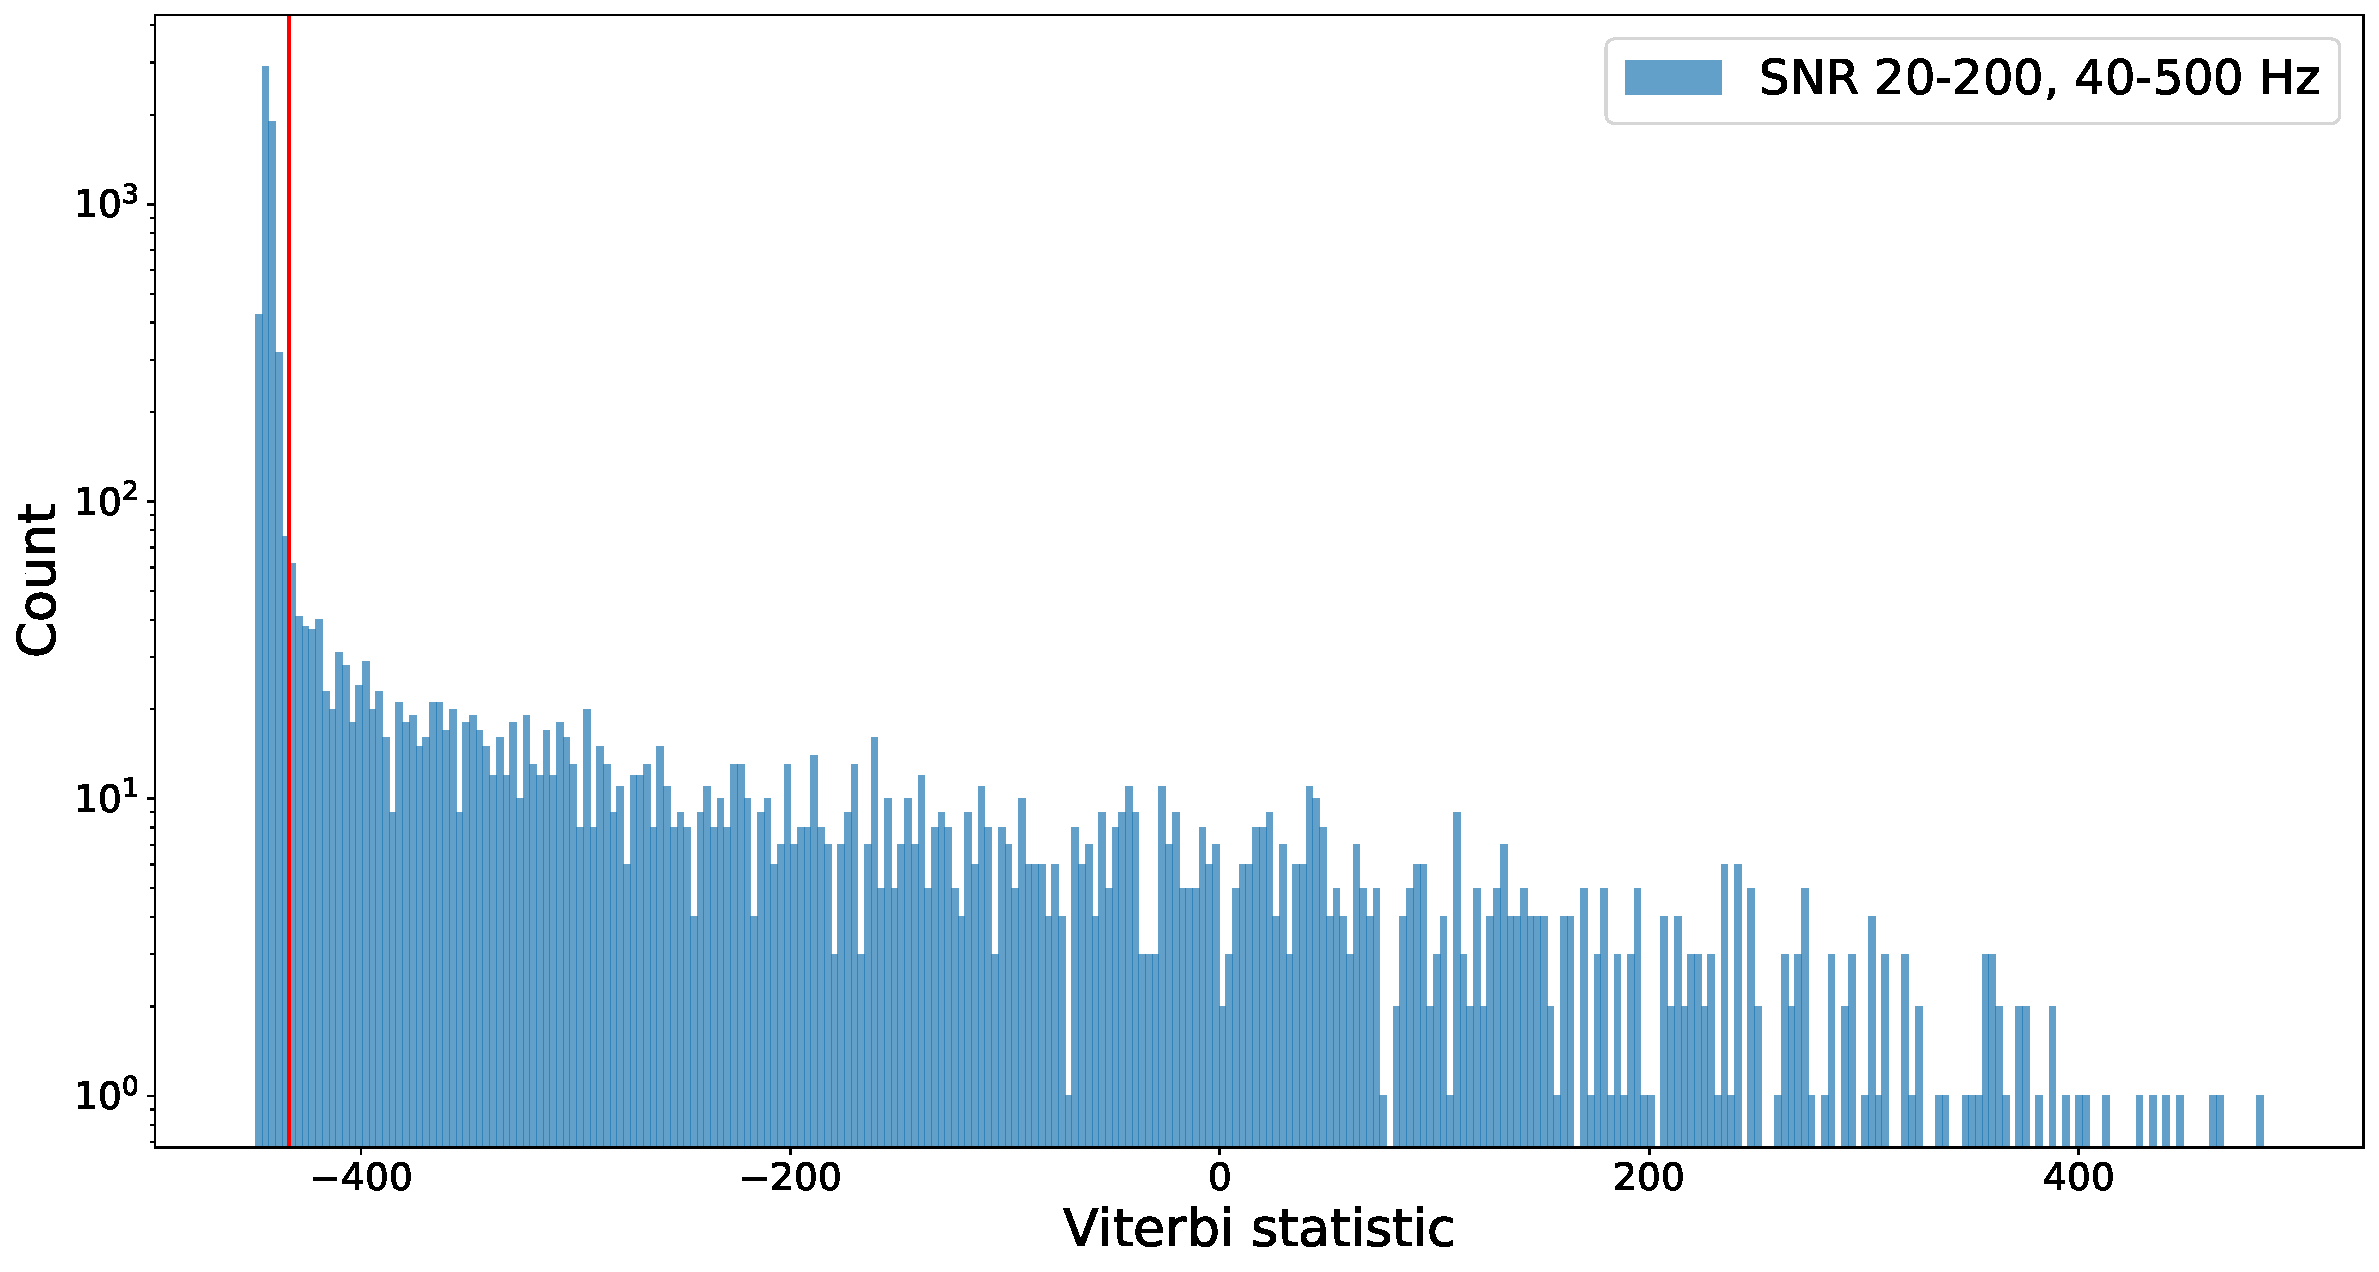
\includegraphics[width=\linewidth]{C5_parameter/viterbi_hist.pdf}
    \caption[Frequency track of injected signal]{ Example frequency and Viterbi track }
    \label{par_est:results:freqtrack}
    
\end{figure}
%
In this case the Viterbi track closely follows the simulated neutrons star frequency track.

The Bayesian analysis described in Sec.~\ref{par_est:bayes} is then run using this Viterbi track as input, this returns the marginal posterior distributions shown in Fig.~\ref{par_est:results:example_posterior}, where the simulated parameters are marked in orange.
In this example, the injected parameter values are within the marginal posterior distributions for all of the parameters.
The frequency is has a width of N in band N \joe{mention all by sky params here}
%
\begin{figure}[pt]

    \centering
    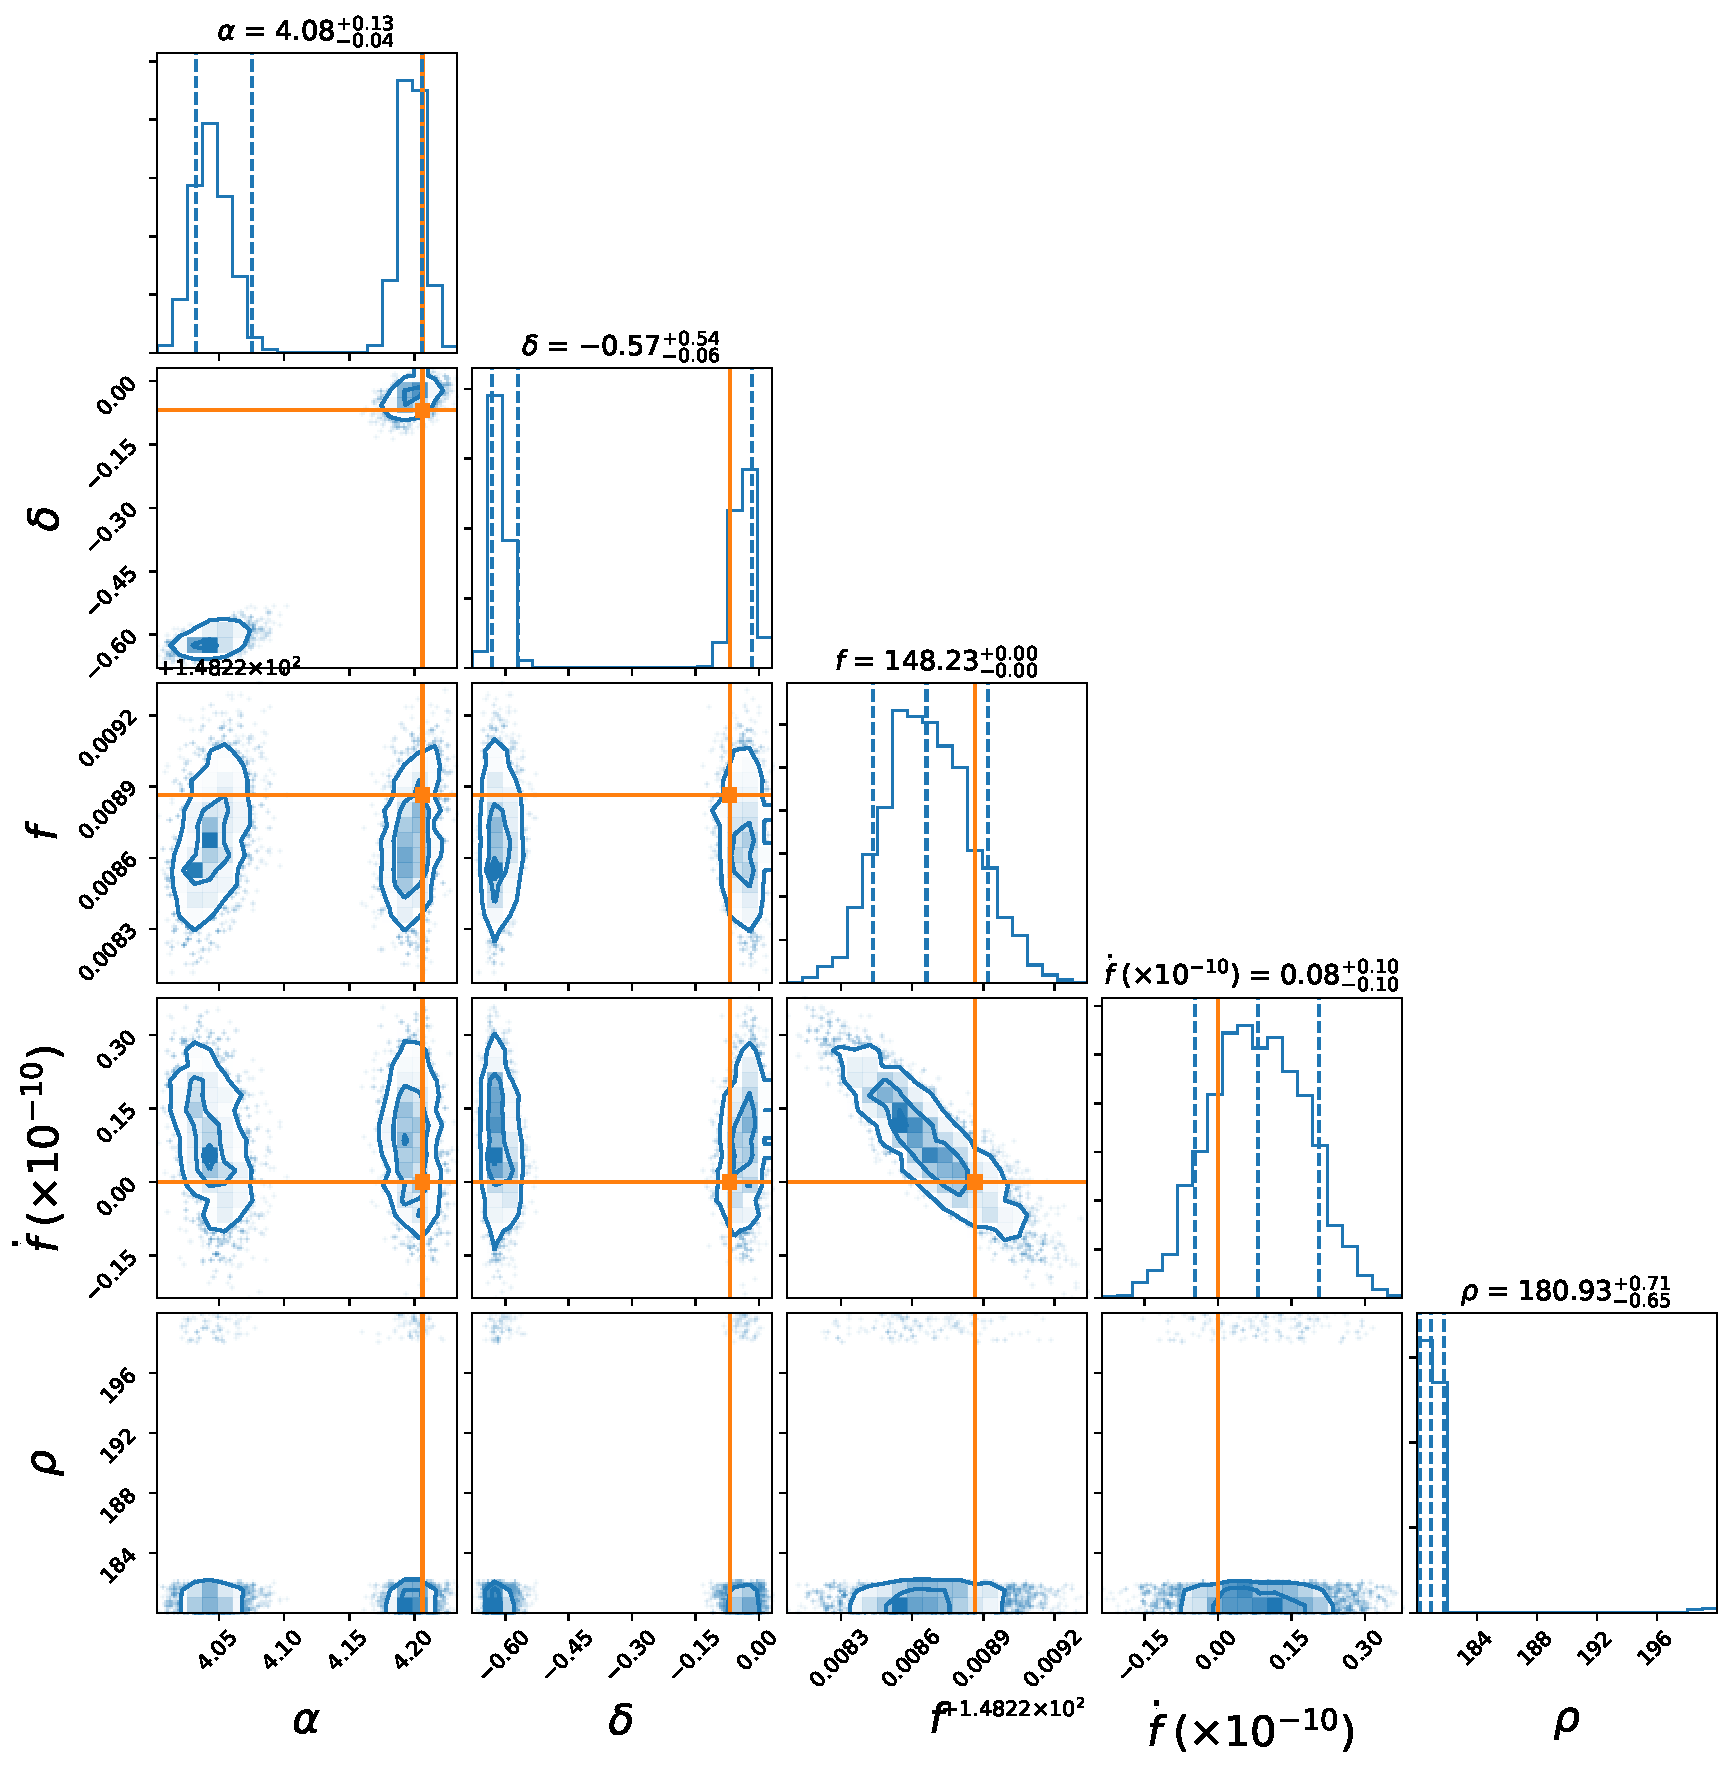
\includegraphics[width=\linewidth]{C5_parameter/cornerplot.pdf}
    \caption[KDE of likelihood in different \gls{SNR} ranges]{This figure shows an example of the posterior distribution of a signal with \gls{SNR} 144. Each panel shows the marginal distributions for each parameter, where the parameters used for the simulation are marked in orange. In this example each of the posteriors match well with the injected parameters, but the sky position is bimodal. }
    \label{par_est:results:example_posterior}
    
\end{figure}
%
It is easier to interpret the distribution of the sky parameters when it is projected onto a skymap, therefore, Fig.~\ref{par_est:results:example_skypos} the parameters $\alpha$ and $\delta$ are shown on a sky projection.
The Viterbi tracks and pulsar frequency tracks used in this analysis are sampled once a day, therefore, we should only see the doppler modulation from the orbit of the earth around the sun.
In the ecliptic frame, i.e. where the $z$ axis is perpendicular to the orbital plane of the earth, for any ecliptic longitude, there are two sky positions at opposite ecliptic latitudes which will return the same frequency track. 
This then means that we would expect the marginal posterior distribution to have two modes on the sky at these two locations, where this can be seen in Fig.~\ref{par_est:results:example_posterier} and \ref{par_est:results:example_skypos}.
The sky position parameters of the neutron star are in the equatorial coordinate system, therefore these have been transformed into the ecliptic frame such that the sky position posteriors easier to interpret.
%
\begin{sidewaysfigure}[p]
    \centering
    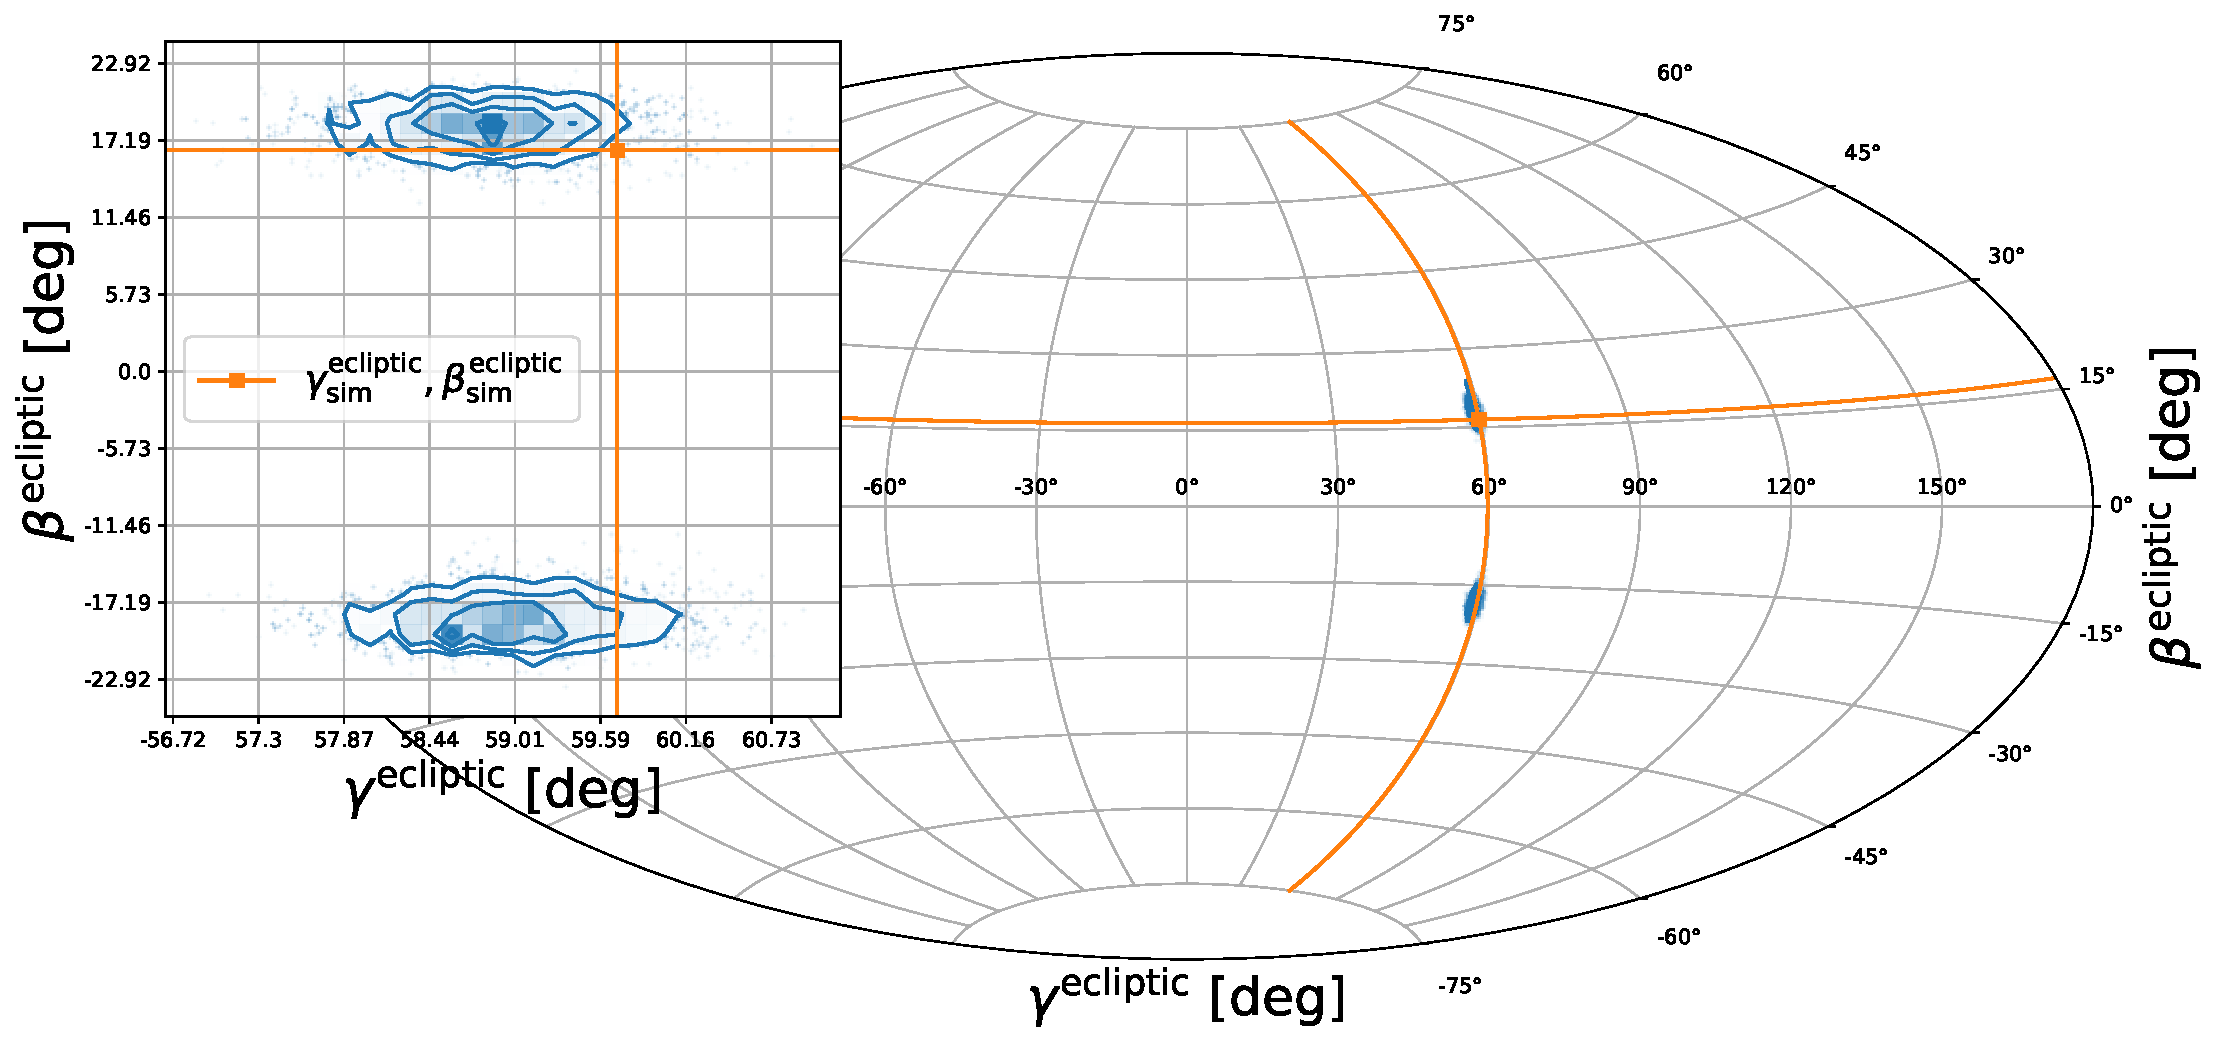
\includegraphics[width=\linewidth]{C5_parameter/skypos_ecliptic.pdf}
    \caption[Example of posterior of sky position]{This figure shows an example of the marginal posterior distribution of the sky position of a signal with \gls{SNR} 144. The coordinates are in the ecliptic frame.}
    \label{par_est:results:example_skypos}
    
\end{sidewaysfigure}
%

\subsection{Simulations}

To test this method, we generate a set of simulations of the spectrograms of pulsar signals as in Sec.~\ref{soap:results} and Sec.~\ref{machine:results}.
In each of these we record the Viterbi track and the pulsar signal parameters $\alpha, \delta, f, \dot{f} , \rho$ associated with each simulation, from which the pulsar track can be generated.
The Viterbi track and the pulsars signal parameters $\alpha, \delta, f, \dot{f}$ is all the information needed to run the Bayesian analysis described in Sec.~\ref{par_est:bayes}.
We generated signals in 50\% of the 0.1 Hz wide sub-bands between between 40 and 500 Hz, with the parameters as described in Tab.~\ref{}. 
This meant that we have 2300 simulated signals which had an \gls{SNR} range between 20 and 200.
However, as the \gls{SNR} of the simulations decreases, the probability of SOAP identifying the signal decreases, therefore, we only want to run the Bayesian parameter estimation on signals which are most likely to be astrophysical.
Therefore, as in Sec.~\ref{soap:results}, we find the false alarm rate, which is the fraction of bands which contain no injection and has a Viterbi statistic which exceeds a given threshold, where this is set to 0\% for this test.
We can then select all of the sub-bands which have a Viterbi statistic above this threshold for further investigation, where with a 0\% false alarm rate we have 2000 \joe{ecaxt number} injections to investigate.
The Viterbi statistics for each of these injections can be seen in Fig.~\ref{par_est:results:all_viterbi}, where the 0\% false alarm value is marked.
%
\begin{figure}
    \centering
    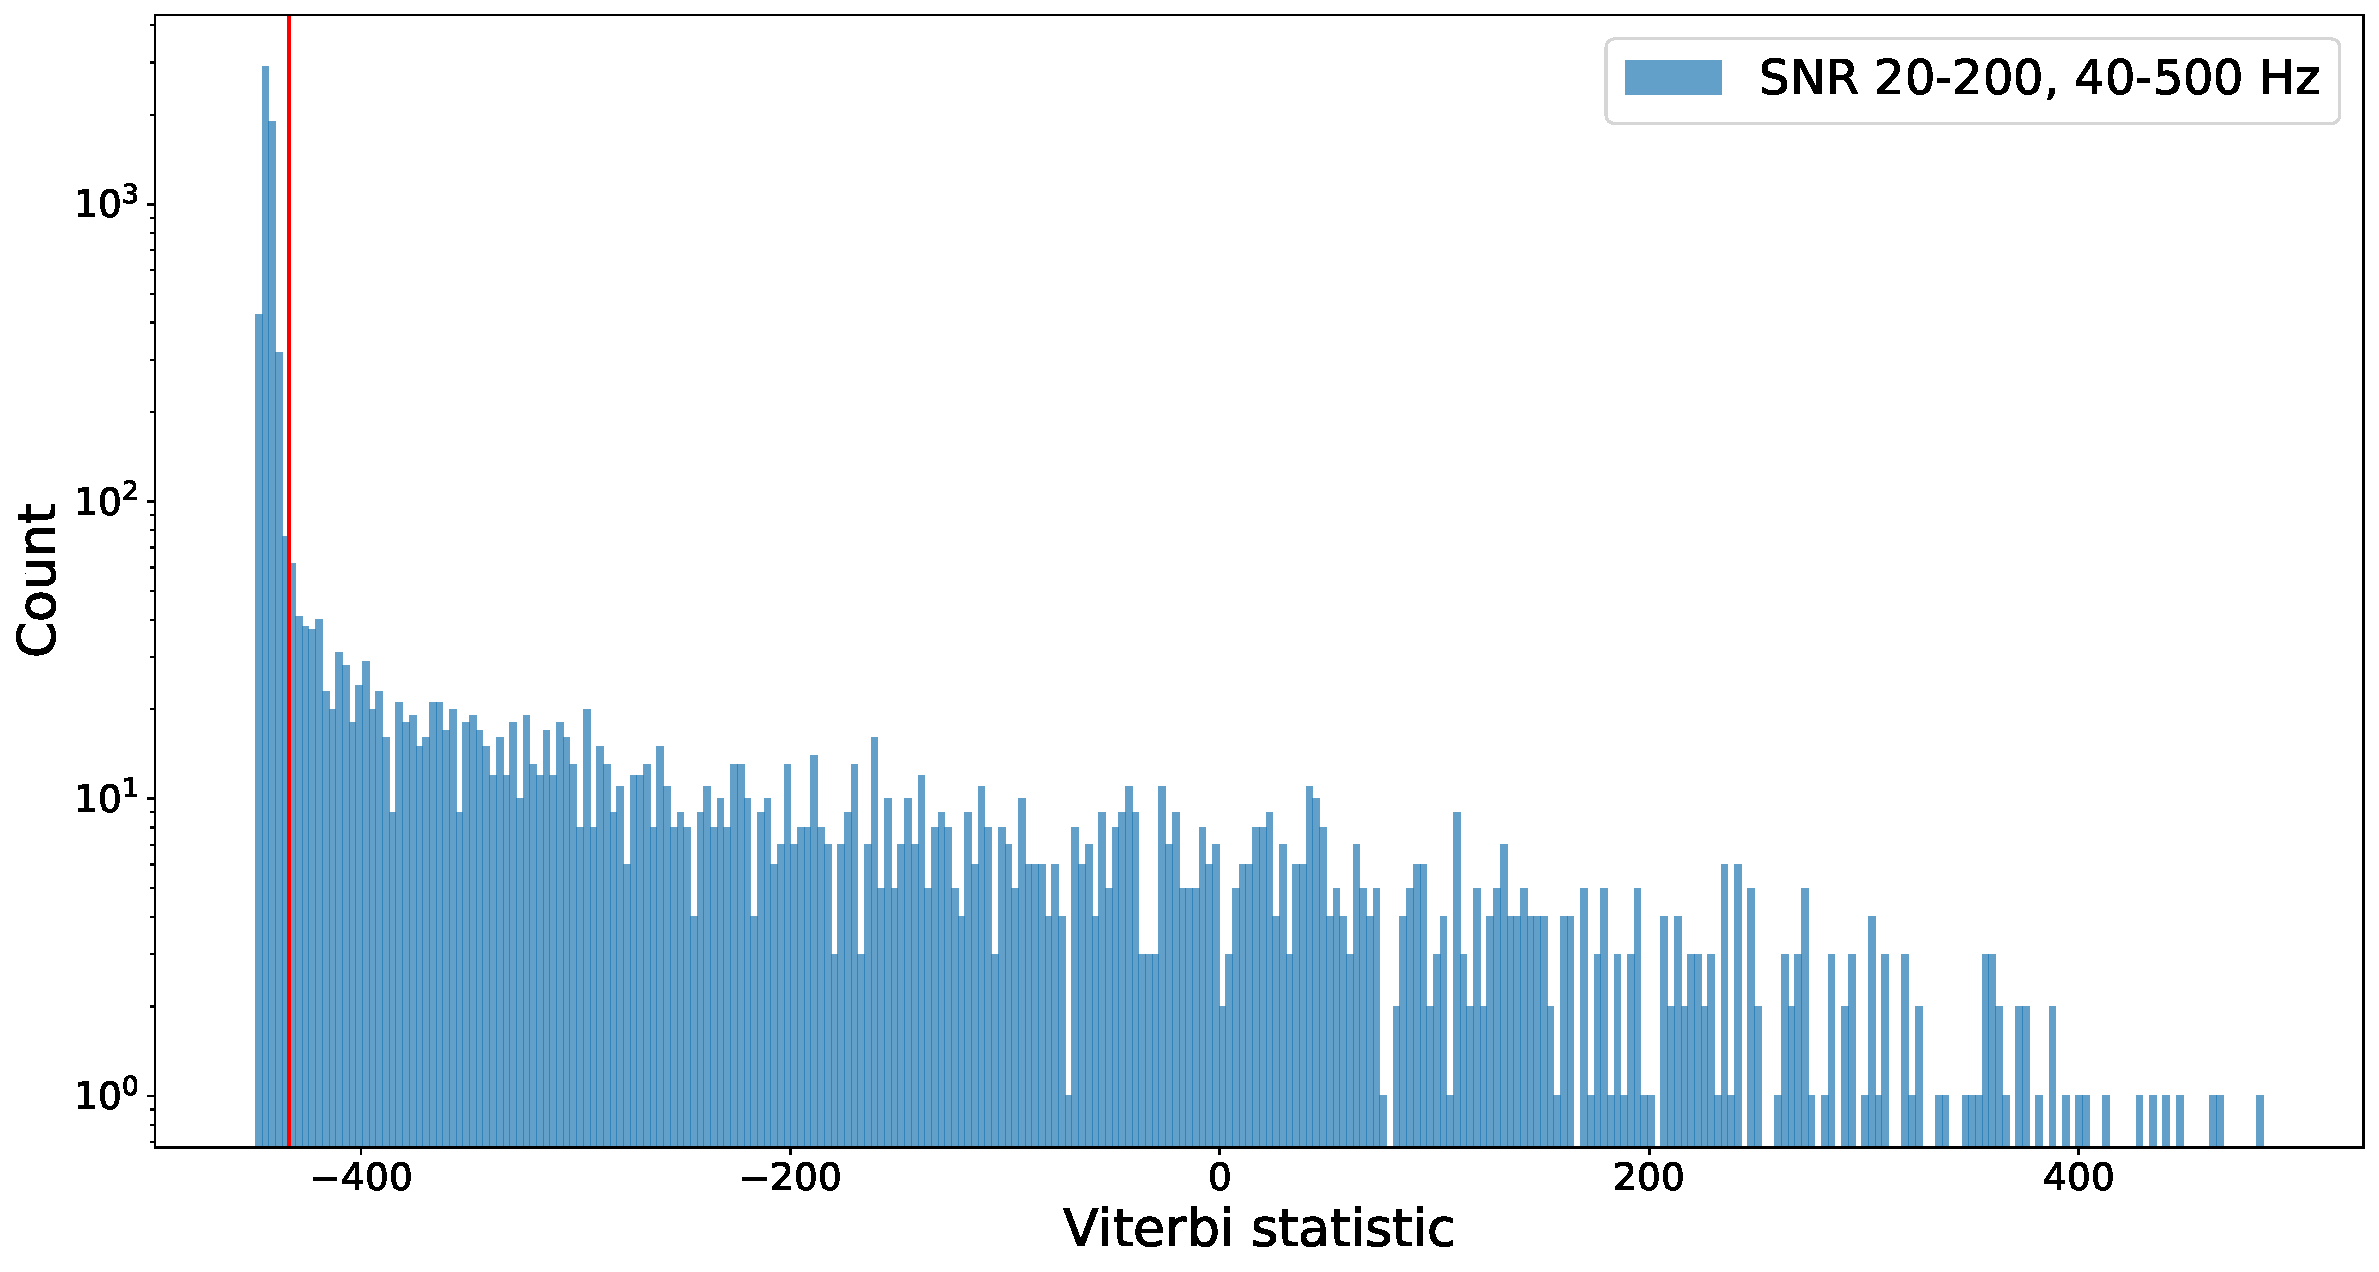
\includegraphics[width=\linewidth]{C5_parameter/viterbi_hist.pdf}
    \caption[All Viterbi statistics]{This figure shows a histogram of the Viterbi statistics from each of the 0.1 Hz wide sub bands in this test. \joe{more}}
    \label{par_est:results:all_viterbi}
\end{figure}


\subsubsection{P-P plot}

The p-p plot is a mechanism to validate the effectiveness of the Bayesian model and computation using many simulations.
From Sec.~\ref{par_est:results} we have the output posterior distribution $p(\bm{\theta} \mid \bm{V}, I)$, or more correctly we have $N$ samples from this distribution $\bm{\theta}_i$, and we have the injected parameters $\bm{\theta}_{\rm{inj}}$.
For each simulation, we can calculate the posterior quantile $q(\theta_{\rm{inj}})$ from the marginal posterior distribution
\begin{equation}
    q(\theta_{\rm{inj}}) = P(\theta_{\rm{inj}} > \theta) = \frac{1}{N} \sum_{i=1}^{N} H(\theta_{\rm{inj}} - \theta_i),
\end{equation}
where $H(x)$ is the Heaviside step function. 
This calculates the fraction of the marginal posterior distribution which has a parameter $\theta$ less than the injected parameter $\theta_{\rm{inj}}$ \citep{cook2006ValidationSoftware}.
If the model and computation of the posterior is valid, then as the number of samples approaches infinity ($N \rightarrow \infty$), the posterior quantile $q(\theta_{\rm{inj}})$ should follow a uniform distribution $[0,1]$ \citep{cook2006ValidationSoftware}.
This then provides a method to check the validity of our analysis.

For each of our simulations we can calculate $q(\theta_{\rm{inj}})$, such that we have values $\bm{q}_{\theta}$, where the fraction of simulations which fall within a given \gls{CI} $C$ is the cumulative distribution of $\bm{q}_{\theta}$, i.e. $P(\bm{q}_{\theta} > C)$, where $C$ ranges between $[0,1]$.
If $q(\theta_{\rm{inj}})$ and therefore $\bm{q}_{\theta}$ follows a normal distribution, then $P(\bm{q}_{\theta} > C) = C$ \citep{cook2006ValidationSoftware}.
Plotting $P(\bm{q}_{\theta} > C)$ against $C$ for each parameter $\theta$, then shows the fraction of simulations which have a $q(\theta_{\rm{inj}})$ within some \gls{CI} $C$, this is known as a p-p plot.

If the analysis is valid, i.e the marginal posterior distributions agree with the injected parameters, then this plot should follow a straight diagonal line, indicated by the black line in Fig.~\ref{par_est:results:ppplot_example}.
If the marginal posterior distribution is shifted to right of the injected parameters, shown in the first panel of Fig.~\ref{par_est:results:ppplot_example}, i.e. the true value lies in the lower tail of the posterior for each simulation, then the p-p plot will show a curve above the diagonal.
Similarly, if the marginal posterior distribution is shifted to left of the injected parameters, shown in the second panel of Fig.~\ref{par_est:results:ppplot_example}, i.e. the true value lies in the upper tail of the posterior for each simulation, then the p-p plot will show a curve below the diagonal. 
If the posterior is under constrained, shown in the third panel of Fig.~\ref{par_est:results:ppplot_example}, i.e. the posterior is wider than the perfectly recovered posterior, then the curve will follow an S shape where the S is below the diagonal at $C < 0$.5 and above the diagonal at $C > 0.5$.
Similarly, if the posterior is over constrained, shown in the fourth panel of Fig.~\ref{par_est:results:ppplot_example},i.e. the posterior is narrower than the perfectly recovered posterior, then the curve will follow an S shape where the S is above the diagonal at $C < 0.5$ and below the diagonal at $C> 0.5$.
%
\begin{figure}[ht]
    \centering
    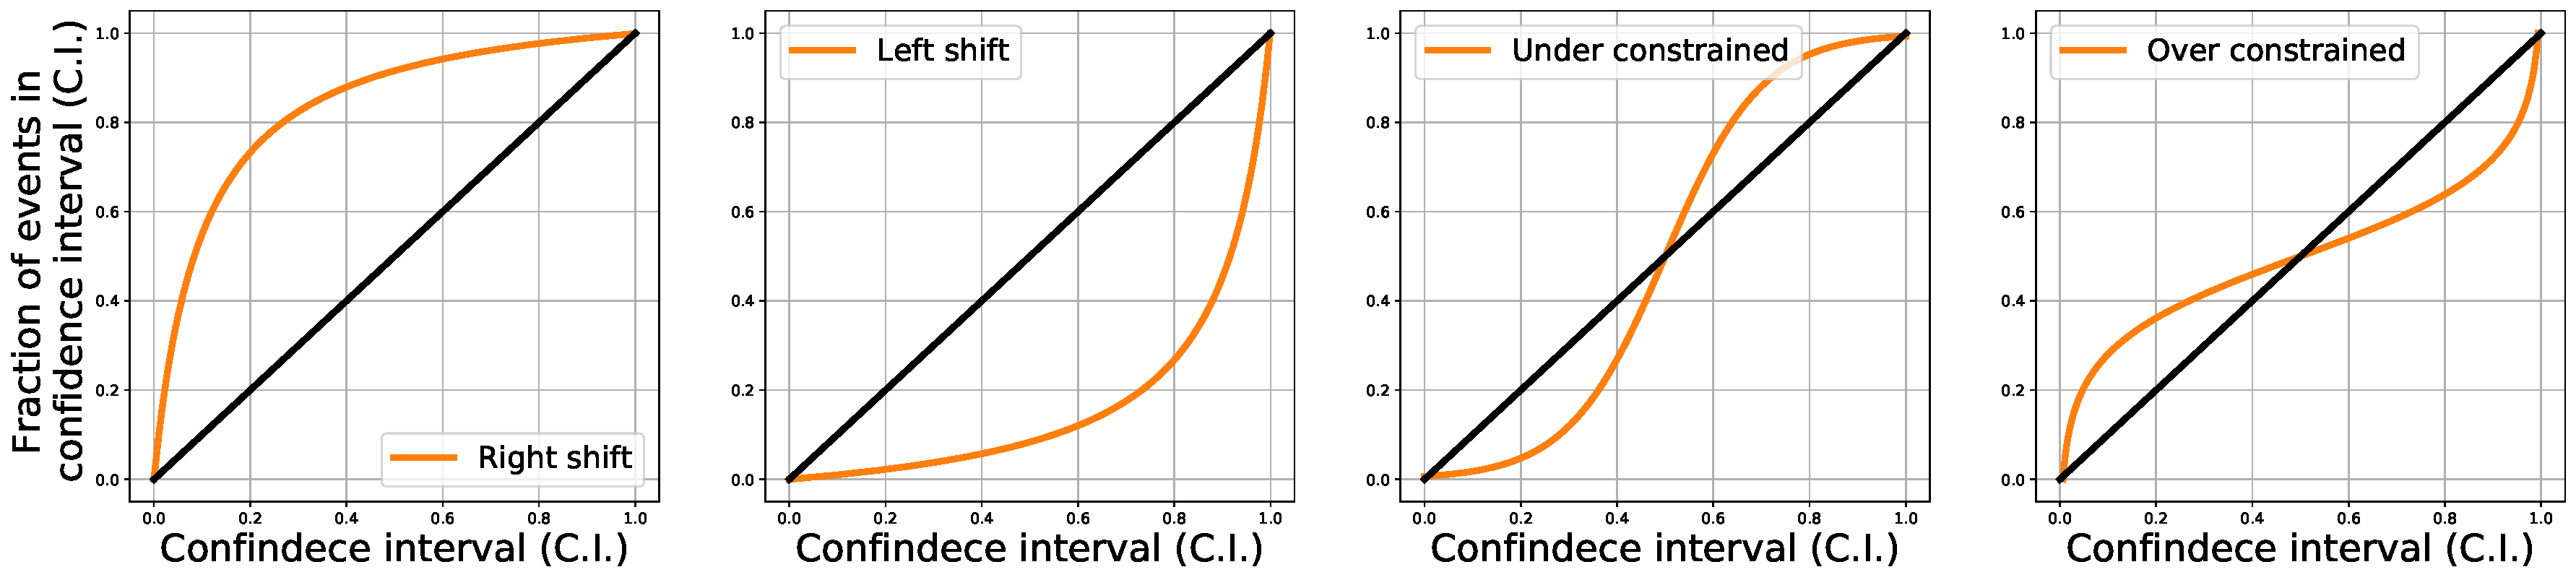
\includegraphics[width=\linewidth]{C5_parameter/ppplot_examples.pdf}
    \caption[p-p plot examples]{This figure shows examples of p-p plots for posterior distributions which are shifted to the right (larger values of the parameter), to the left (smaller values of the parameter) and over and under constrained posteriors. The black curve shows the p-p plot when the posterior distribution is perfectly recovered, i.e. the confidence intervals follow a uniform distribution.}
    \label{par_est:results:ppplot_example}
\end{figure}

Using this information, we can look at the p-p plot for the 2000 \joe{check} simulations in this test, which is shown in Fig.~\ref{par_est:results:ppplot}.
We can see that for the parameters $f$ and $\dot{f}$ we recover an under constrained posterior distribution, which implies that we are under confident about our estimation of the parameters.
For the \gls{SNR} parameter $\rho$, the recovered posterior is shifted to the right, i.e. we assume higher \glspl{SNR} than perfectly recovered distribution.
For the right ascension parameter $\alpha$, we can see that we are both shifted to the right and is over constrained, therefore, we are overconfident that the estimation of this parameter is correct.
For the declination parameters $\delta$, the posterior distribution is both over constrained and shifted to the right, this is largely as the posterior is bi-modal. 
%
\begin{figure}[ht]
    \centering
    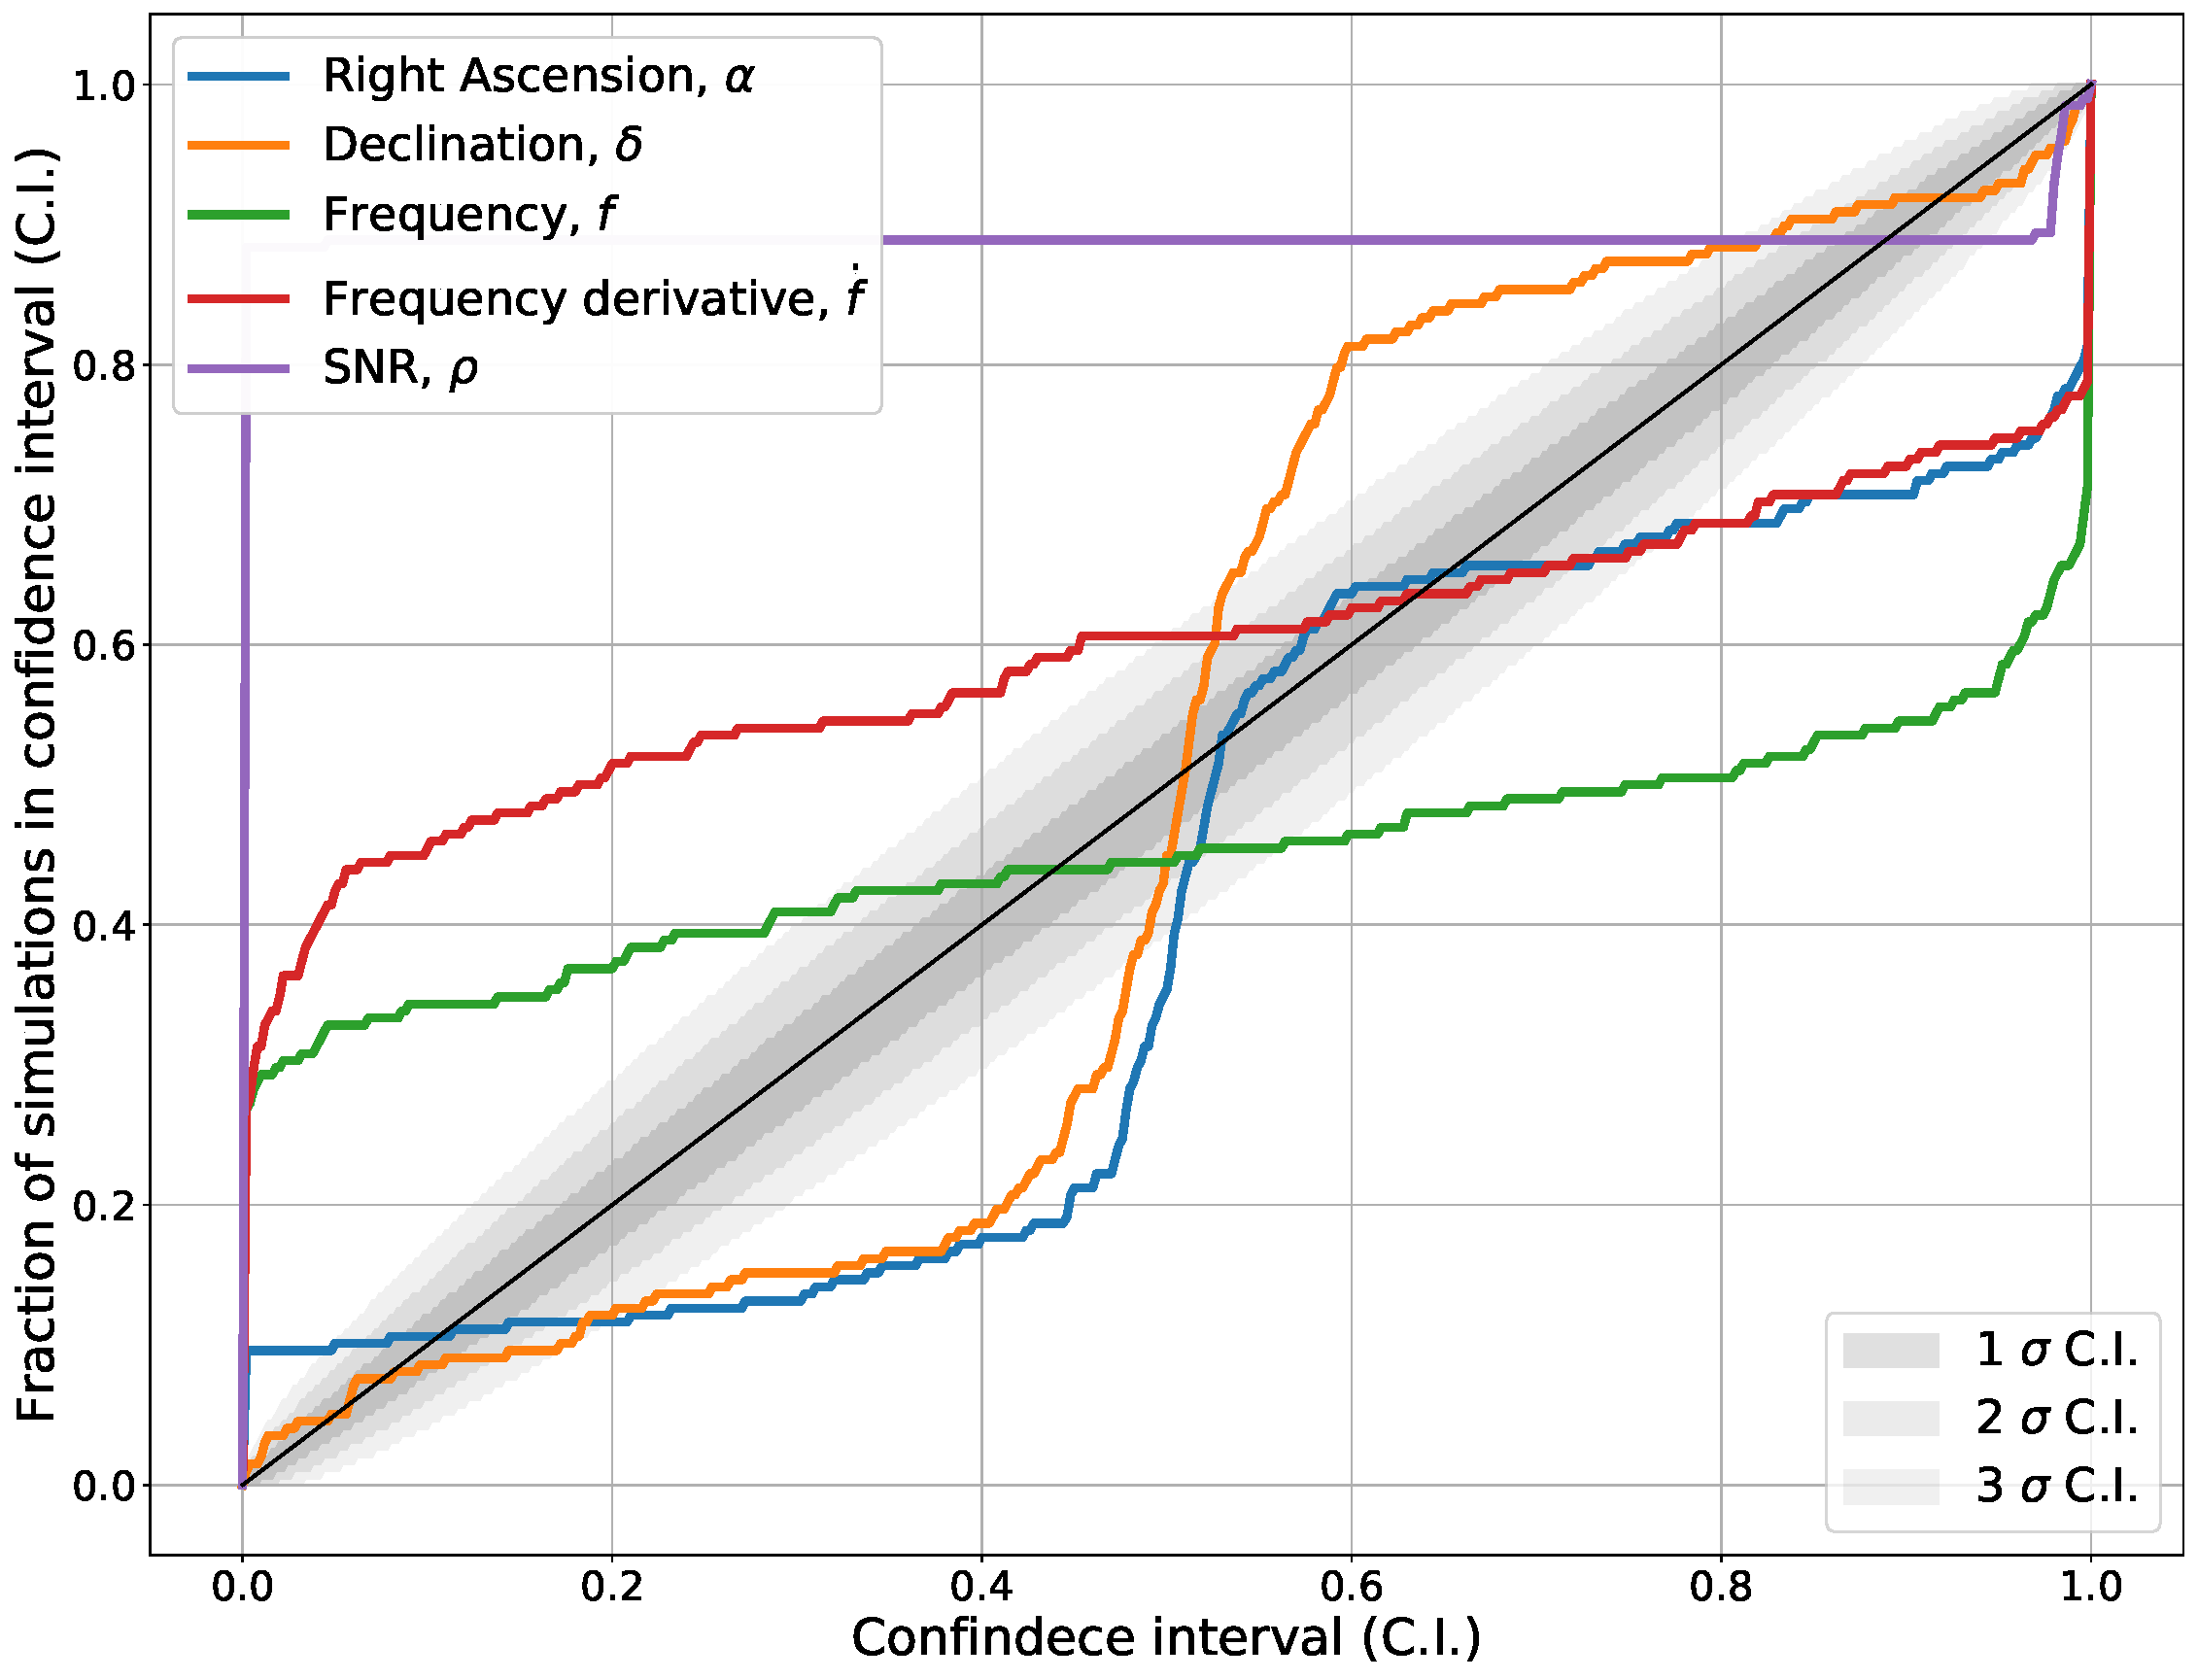
\includegraphics[width=\linewidth]{C5_parameter/ppplot.pdf}
    \caption[p-p plot for the CW simulations]{This figure shows the p-p plot for the 2000 `detected' signals by SOAP in the test described in Sec.~\ref{par_est:results}. \joe{need to figure out the confidece interval of the confidence interval}\joe{more}}
    \label{par_est:results:ppplot}
\end{figure}

The over constrained posterior distributions are due to the assumption that the frequency track elements are independent in the likelihood described in Sec.~\ref{par_est:bayes:likelihood}.
These elements are in fact dependent i.e. 
\joe{say why this doesnt work and how it could be improved}

\subsubsection{Sky area at given confidence interval}

If we assume that the estimated posterior distribution is correct, i.e. it is not under constrained or shifted, then we can estimate the area of the sky which this method can localise the source to. 
To do this we can use the posterior samples to draw a contour on the 2d sky map where the posterior contains 90\% of the probability.
This area contained within this contour is then the sky area which this method can localise the source to at 90\% confidence.
An example of this can be seen in Fig.~\ref{}.

This sky area can be calculated for all of the simulations described in Sec.~\ref{par_est:results}, where Fig.~\ref{par_est:results:sky_area} shows a histograms of all of the sky areas at 90\% confidence in square degrees.
%
\begin{figure}[ht]
    \centering
    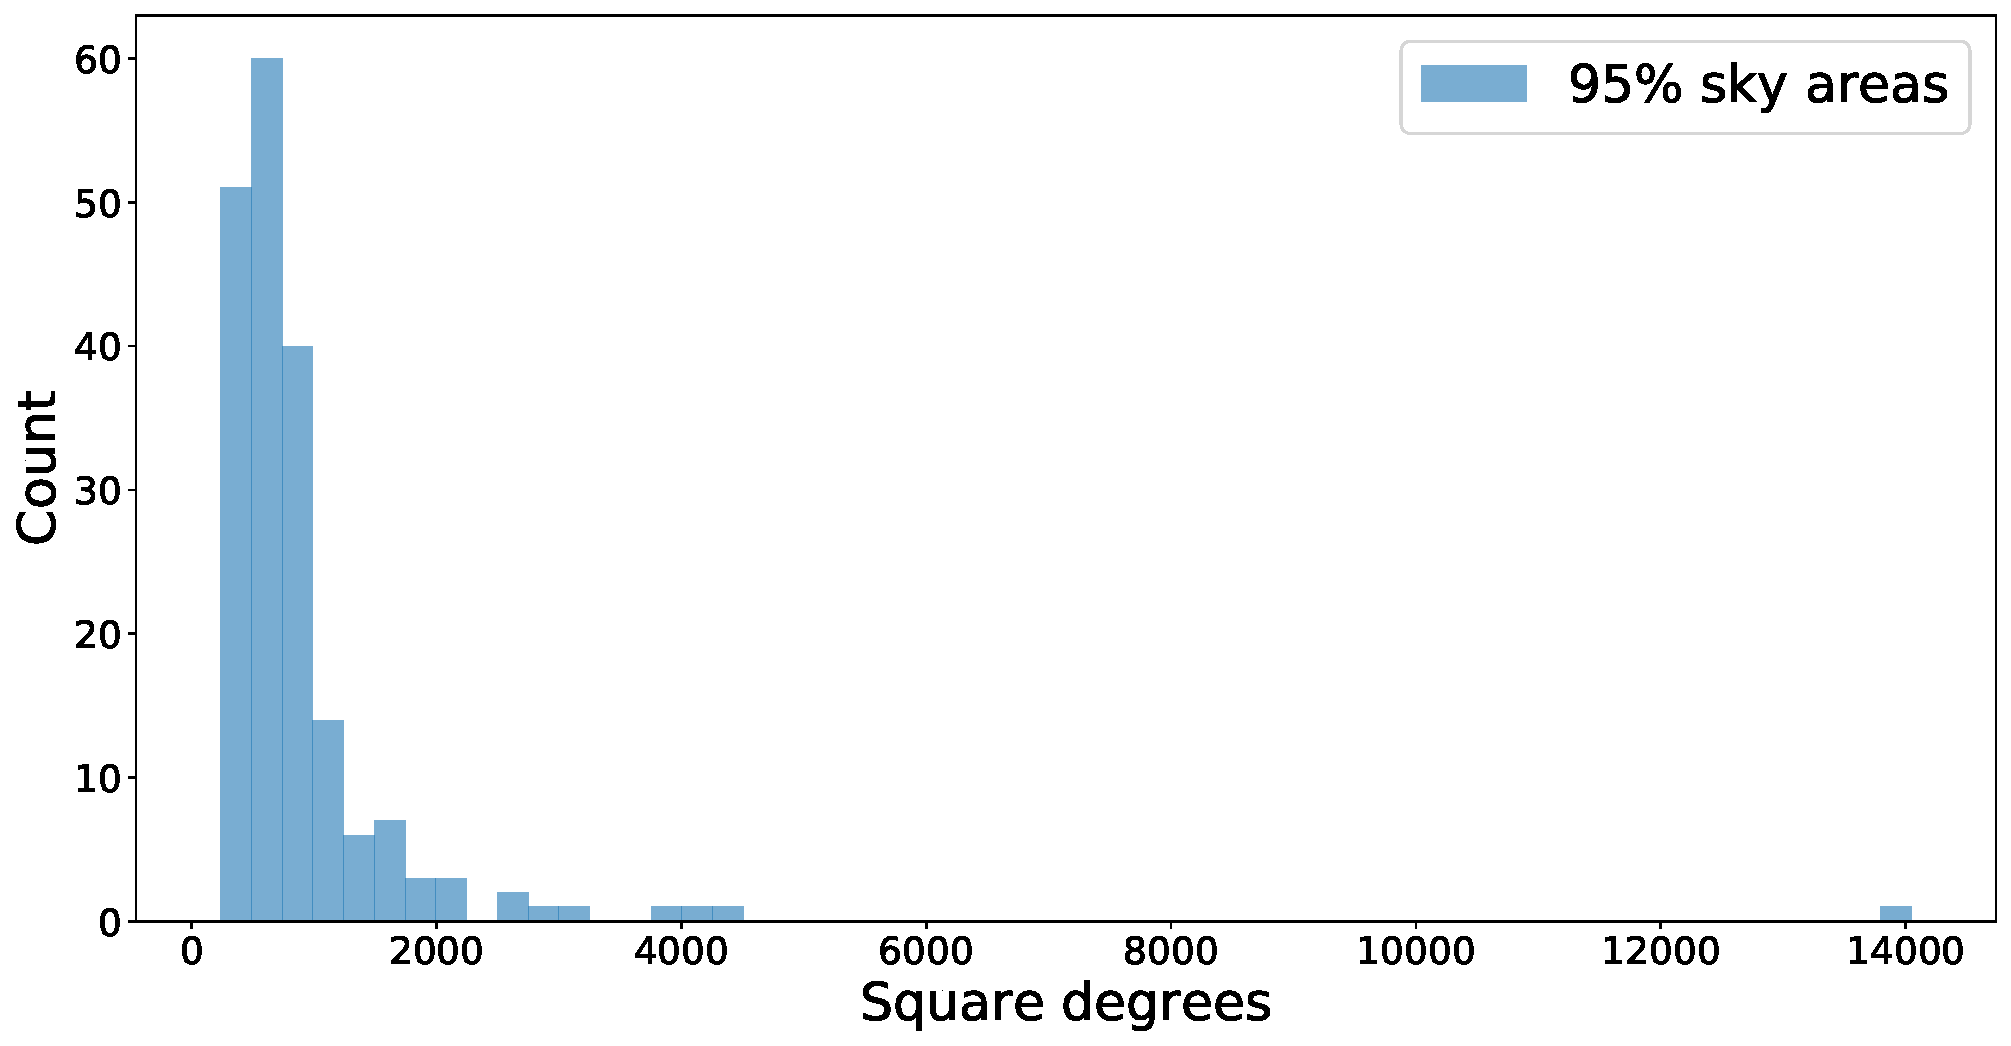
\includegraphics[width=\linewidth]{C5_parameter/sky_area_hist.pdf}
    \caption[p-p plot for the CW simulations]{This figure shows the p-p plot for the 2000 `detected' signals by SOAP in the test described in Sec.~\ref{par_est:results}. \joe{more}}
    \label{par_est:results:sky_Area}
\end{figure}



\joe{say what reduction in sky area is useful for passing on to future searches}
